\documentclass{sig-alternate}
\usepackage[utf8]{inputenc}

\usepackage{amsmath,amssymb}
\usepackage{amsrefs}
\usepackage[usenames,dvipsnames]{color}
\usepackage{stmaryrd}
\usepackage{enumerate}
\usepackage[algoruled,vlined,english,linesnumbered]{algorithm2e}
\usepackage[pdfpagelabels,colorlinks=true,citecolor=blue]{hyperref}
\usepackage{comment}
\usepackage{multirow}
\usepackage{tikz}

\newcommand{\noopsort}[1]{}
\DeclareMathOperator{\NP}{NP}
\DeclareMathOperator{\Hom}{Hom}
\DeclareMathOperator{\End}{End}
\DeclareMathOperator{\GL}{GL}
\DeclareMathOperator{\val}{val}
\DeclareMathOperator{\pr}{pr}
\DeclareMathOperator{\tr}{Tr}
\DeclareMathOperator{\com}{Com}
\DeclareMathOperator{\Grass}{Grass}
\DeclareMathOperator{\Lat}{Lat}
\DeclareMathOperator{\round}{round}

\begin{document}

\newtheorem{theo}{Theorem}[section]
\newtheorem{lem}[theo]{Lemma}
\newtheorem{prop}[theo]{Proposition}
\newtheorem{cor}[theo]{Corollary}
\newtheorem{quest}[theo]{Question}
%\theoremstyle{definition}
\newtheorem{rem}[theo]{Remark}
\newtheorem{ex}[theo]{Example}
\newtheorem{deftn}[theo]{Definition}
\newtheorem{rmk}[theo]{Remark}

\newcommand{\N}{\mathbb N}
\newcommand{\Z}{\mathbb Z}
\newcommand{\Zp}{\Z_p}
\newcommand{\Q}{\mathbb Q}
\newcommand{\Qp}{\Q_p}
\newcommand{\Fp}{\mathbb{F}_p}
\newcommand{\R}{\mathbb R}
\renewcommand{\O}{\mathcal O}
\newcommand{\OK}{\mathcal{O}_K}
\newcommand{\XX}{\mathbf X}
\newcommand{\trans}{{}^{\text t}}
\newcommand{\T}{\mathcal{T}}

\renewcommand{\prec}{\text{\rm prec}}

\newcommand{\id}{\textrm{id}}
\newcommand{\Epi}{\textrm{Epi}}
\renewcommand{\c}{\text{\rm c}}

\newcommand{\detp}{\text{\rm det}'}
\newcommand{\DI}{\text{\rm DI}}
\newcommand{\II}{\text{\rm II}}

\newcommand{\lb}{\ensuremath{\llbracket}}
\newcommand{\rb}{\ensuremath{\rrbracket}}
\newcommand{\lp}{(\!(}
\newcommand{\rp}{)\!)}
\newcommand{\col}{\: : \:}

\def\todo#1{\ \!\!{\color{red} #1}}
\definecolor{purple}{rgb}{0.6,0,0.6}
\def\todofor#1#2{\ \!\!{\color{purple} {\bf #1}: #2}}

\def\binom#1#2{\Big(\begin{array}{cc} #1 \\ #2 \end{array}\Big)}

\title{About p-adic stability in linear algebra}

\numberofauthors{3}
\author{
\alignauthor Xavier Caruso\\
  \affaddr{Universit\'e Rennes 1}\\
  \email{\normalsize \textsf{xavier.caruso@normalesup.org}}
\alignauthor Tristan Vaccon\\
  \affaddr{Universit\'e Rennes 1}\\
  \email{\normalsize \textsf{tristan.vaccon@univ-rennes1.fr}}
\alignauthor David Roe \\
  \affaddr{University of Calgary}\\
  \email{\normalsize \textsf{roed.math@gmail.com}}
}

\maketitle

\begin{abstract}
Based on the framework developed in \cite{caruso-roe-vaccon:14a}, we study 
the $p$-adic stability of standard operations on matrices and vector 
spaces. 
%We observe in particular that generic algorithms --- which are 
%designed to work over an arbitrary field --- are generally very 
%unstable.
\end{abstract}

\vspace{1mm}
 \noindent
 {\bf Categories and Subject Descriptors:} \\
\noindent I.1.2 [{\bf Computing Methodologies}]:{~} Symbolic and Algebraic
  Manipulation -- \emph{Algebraic Algorithms}

 \vspace{1mm}
 \noindent
 {\bf General Terms:} Algorithms, Theory

 \vspace{1mm}
 \noindent
 {\bf Keywords:} $p$-adic precision
\medskip

\section{Introduction}

For about twenty years, the use of $p$-adic methods in symbolic 
computation was gaining more and more popularity: they were succesfully 
used for instance 
to compute compose products of polynomials 
\cite{boston-gonzalez-perdry-schost:05a}, 
to produce hyperelliptic curves of genus $2$ with complex multiplication 
\cite{gaudry-houtmann-weng-ritzenthaler-kohel:06a},
to compute isogenies between elliptic curves \cite{lercier-sirvent:08a} 
and, last but not least,
to count points on certain varieties (mainly curves) using $p$-adic 
cohomologies (\emph{cf} \cite{kedlaya:01a,lauder:04a} and many
followers).
However, a general framework allowing a precise study of $p$-adic 
precision --- which is a main issue we encounter when trying to work 
with $p$-adic numbers --- was designed only recently in 
\cite{caruso-roe-vaccon:14a}. 

\todo{Rewrite the introduction}

\begin{comment}
The present paper, which may be considered as a continuation of 
\cite{caruso-roe-vaccon:14a}, aims at using the theory of \emph{loc. 
cit.} in order to analyse the $p$-adic stability of many standard 
algorithms for computing with basic algebraic structures: numbers, 
matrices, univariate polynomials and vector spaces. For each considered 
algorithm, we will follow the same protocol: 
first, we will compute the theoretical loss of precision of the 
underlying question using the framework of \cite{caruso-roe-vaccon:14a} 
and then compare it to those observed in available implementations in 
\textsc{pari} \cite{pari}, \textsc{magma} \cite{magma} and/or 
\textsc{sage} \cite{sage}.

The conclusion of our analysis is that generic algorithms which are 
designed to work over an arbitrary field are often quite unstable. Very 
roughly, denoting by $D$ the number of divisions performed by the 
algorithm under analysis and by $q$ the cardinality of the residue 
field, it appears that the numbers of lost digits is about $O(\frac D 
q)$ whereas the theoretical loss of precision is closer than $O(\log_q 
D)$ --- and sometimes even $O(1)$. We would like to underline in 
particular that the instability phenomema are much more apparent when 
the residue field is small. It is the reason why we will always take
$K = \Q_2$ is our examples.
\end{comment}

\medskip

\noindent
{\bf Organization of the paper.}
The section \ref{sec:theory} introduces the theory of ultrametric 
precision developped in \cite{caruso-roe-vaccon:14a} and completes it 
on a technical point. In \S \ref{sec:matrices}

The analysis of standard algorithms are treated in 
the next sections: \S\S \ref{sec:numbers}--\ref{sec:vectorspaces} are 
successively devoted to the case of numbers, matrices, univariate 
polynomials, multivariate polynomials and finally vector spaces.

\medskip

\noindent
{\bf Notations.}
Throughout the paper, the letter $K$ will refer to a \emph{complete 
discrete valuation field of characteristic $0$}, that is either a finite 
extension of the field of $p$-adic numbers $\Qp$ or a field of Laurent 
series over a field of characteristic $0$. We denote by $\val : K \to \Z 
\cup \{+\infty\}$ of $K$ --- it is the $p$-adic valuation when $K = \Qp$ 
and the usual valuation of a Laurent series when $K = k((t))$ --- and by 
$\Vert \cdot \Vert$ the corresponding norm.

\section{The theory of p-adic precision}
\label{sec:theory}

The aim of this section is to summerize briefly the content of 
\cite{caruso-roe-vaccon:14a} and complete it on certain points.

\subsection{Lattices as precision data}

Roughly speaking, the main proposal of \cite{caruso-roe-vaccon:14a} is 
to use lattices to track precision when computing with elements lying in 
vector spaces over $K$.

To make this sentence more explcit, let us consider be a finite 
dimensional\footnote{The framework of \cite{caruso-roe-vaccon:14a} is 
actually those of Banach spaces. However we will not need infinite 
dimensional spaces in the present paper.} normed vector space $E$ 
defined over $K$. We use the notation $\Vert \cdot \Vert_E$ for the norm 
on $E$ and $B^-_E(r)$ (resp. $B^{\phantom -}_E(r)$) for the open (resp. 
closed) ball of radius $r$ centered at the origin. A lattice $L \subset 
E$ is, by definition, a sub-$\O_K$-module which generates $E$ over $K$. 
Since we are working in a ultrametric world, the balls $B^{\phantom 
-}_E(r)$ and $B^-_E(r)$ are examples of lattices. Actually, lattices 
should be thought as special neighborhoods of $0$ and therefore are good 
candidates to model precision data. Moreover, as revealed in 
\cite{caruso-roe-vaccon:14a}, they behave quite well under (strictly) 
differentiable maps:

\begin{prop}
\label{prop:precision}
Let $E$ and $F$ be two finite dimensional normed vector spaces over $K$ 
and $f : U \rightarrow F$ be a function defined on an open subset $U$ of 
$E$. We assume that $f$ is differentiable at some point $v_0 \in U$ and 
that the differential $f'(v_0)$ is surjective.
Then, for all $\rho \in (0, 1]$, there exists a positive real
number $\delta$ such that, for all $r \in (0, \delta)$, any lattice
$H$ such that $B^-_E(\rho r) \subset H \subset B^{\phantom -}_E(r)$ 
satisfies:
\begin{equation}
\label{eq:firstorder}
f(v_0 + H) = f(v_0) + f'(v_0) (H).
\end{equation}
\end{prop}

Proposition \ref{prop:precision} can be rephrased in terms of precision 
as follows: if the input $v_0$ is known at precision $H$, then $f(v_0)$ 
is known up to $f'(v_0)(H)$ and this precision is optimal. Optimality is 
reflected by the equality sign in Eq.~\eqref{eq:firstorder}.

In \cite{caruso-roe-vaccon:14a}, we also explained that if the function 
$f$ is locally analytic, then the constant $\delta$ appearing in
Proposition \ref{prop:precision} can be made explicit in terms of the
growing function $\Lambda(f)$ of $f$ defined by:
$$\textstyle \Lambda(f)(v) = 
\log \big( \sup_{h \in B^-_E(e^v)} \Vert 
f(h) \Vert \big)$$
with the convention that $\Lambda(f)(v) = +\infty$ if $f$ does not
converge on $B^-_E(e^v)$.
We refer to \cite[Proposition 3.12]{caruso-roe-vaccon:14a} for the
precise statement and seek here to state the particular case of
polynomial functions. A function $f : E \to F$ is said \emph{polynomial} 
if it is coordinate-wise given by multivariate polynomials in any 
(equivalently all) system of coordinates associated to orthonormal 
basis.

\begin{prop}
\label{prop:precision2}
We keep the notations of Proposition \ref{prop:precision} and assume 
in addition that $f$ is polynomial. Let $C$ be a positive real
number such that $B_F(1) \subset f'(v_0)(B_E(C))$. 
Then Proposition \ref{prop:precision} holds with $\delta = C \cdot
\rho^{-1}$.
\end{prop}

\subsection{A bound on a growing function}
\label{ssec:boundLambdaf}

In the next sections, we will compute the derivative of several standard 
operations and remark that it sometimes has a simple expression in term 
of the input and the output. In other terms, the function $f$ modeling
such an operation satisfies a differential equation of the form
$f' = g \circ (f, \id)$
where $g$ is a given --- and hopefully rather simple --- function. The 
aim of this subsection is to study this differential equation and to 
derive from it some bounds on the growing function $\Lambda(f)$. 
\emph{In the following, we shall always assume that $K$ has 
characteristic $0$.}

We actually generalize a bit the setting above and consider the 
differential equation:
\begin{equation}
\label{eq:diffequah}
f' = g \circ (f, h).
\end{equation}
Here $g$ and $h$ are known locally analytic functions and $f$ is the 
unknown, which is assumed to be locally analytic as well. The function
$f$ goes from $U$ to $V$, two open subsets in two finite dimensional
normed vector spaces $E$ 
and $F$ respectively. The function $h$ goes from $U$ to $W$ where $W$
is again an open subset in a $K$-Banach space $G$. Consequently, $g$
goes from $V \times W$ to the vector space $\Hom(E,F)$ gathering
all (continuous) linear applications $E \to F$.
In what follows, we always assume that $V$ and $W$ contains the origin, 
$f(0) = 0$, $h(0) = 0$ and $g(0) \neq 0$. There assumptions are harmless 
for two reasons: first, we can always shift $f$ and $h$ (and $g$ 
accordingly) so that they both vanish at $0$ and second, in order to 
apply Proposition \ref{prop:precision2}, the derivative $f'(0)$ 
needs to be surjective and therefore \emph{a fortiori} nonzero.

We assume that we are given in addition two nondecreasing convex 
functions $\Lambda_g$ and $\Lambda_h$ such that $\Lambda(g) \leq 
\Lambda_g$ and $\Lambda(h) \leq \Lambda_h$. We suppose further that 
there exists $\nu$ such that $\Lambda_g$ is constant on the interval 
$]{-}\infty, \nu]$\footnote{We note that this assumption is fullfiled if 
we take $\Lambda_g = \Lambda(g)$ because we have assumed that $g(0)$ 
does not vanish.}. We introduce the functions $\tau_\nu$ and $\Lambda_f$ 
defined by:
$$\begin{array}{rll}
&\tau_\nu(x) = x & \text{if } x \leq \nu \\
& \hphantom{\tau_\nu(x)} = {+} \infty & \text{otherwise} \medskip \\
\text{and} &
\multicolumn{2}{l}{\Lambda_f(x) = 
  \tau_\nu \circ (\id + \Lambda_g \circ \Lambda_h)(x + \alpha)}
\end{array}$$
where $\alpha$ is a real number satisfying $\Vert n! \Vert \geq 
e^{-\alpha n}$ for all $n$. A suitable value for $\alpha$ is $\alpha = - 
\frac p {p-1} \cdot \log \Vert p \Vert > 0$ where $p$ denotes the 
characteristic of the residue field and where, by convention, the above 
expression equals $0$ if $p = 0$.
The next Proposition is proved in Appendix \ref{app:proof}.

\begin{prop}
\label{prop:boundLambdaf}\label{PROP:BOUNDLAMBDAF}
We have $\Lambda(f) \leq \Lambda_f$.
\end{prop}

\begin{figure}
\null \hfill
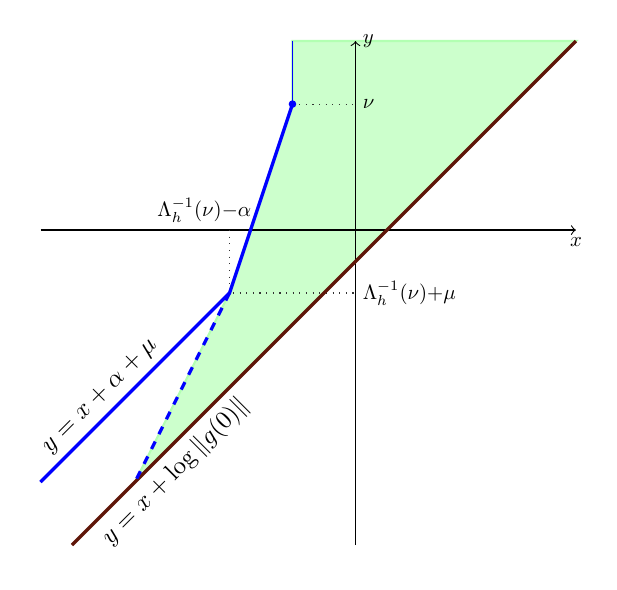
\begin{tikzpicture}[scale=0.8]
\draw[thick,green!30,fill=green!20] 
   (-2,-1)--(-1,2)--(-1,3)--(3.5,3)
 --(2.5,2)--(-3.5,-4)--cycle;
\draw[->] (-5,0)--(3.5,0);
\draw[->] (0,-5)--(0,3);
\node[below, scale=0.75] at (3.5,0) { $x$ };
\node[right, scale=0.75] at (0,3) { $y$ };
\draw[black!80,dotted] (-1,2)--(0,2);
\node[right,scale=0.75] at (0,2) { $\nu$ };
\draw[black!80,dotted] (-2,0)--(-2,-1)--(0,-1);
\node[above,scale=0.75] at (-2.4,0) { $\Lambda_h^{-1}(\nu){-}\alpha$ };
\node[right,scale=0.75] at (0,-1) { $\Lambda_h^{-1}(\nu){+}\mu$ };
\draw[Blue,very thick] (-5,-4)--(-2,-1)--(-1,2);
\fill[Blue] (-1,2) circle (0.06);
\draw[Blue] (-1,2)--(-1,3);
\draw[Sepia, very thick] (-4.5,-5)--(3.5,3);
\draw[Blue, very thick,dashed] (-2,-1)--(-3.5,-4);
\node[below right,rotate=45,scale=0.9] at (-4.3,-4.8) 
  { $y = x + \log \Vert g(0) \Vert$ };
\node[above right,rotate=45,scale=0.9] at (-4.8,-3.8) 
  { $y = x + \alpha + \mu$ };
\end{tikzpicture}
\hfill \null

\caption{Admissible region for the graph of $\Lambda(f)$}
\label{fig:area}
\end{figure}

Figure \ref{fig:area} illustrates Proposition \ref{prop:boundLambdaf}. 
The blue plain line represents the graph of the function $\Lambda_f$. A 
quick computation shows that, on a neighborhood of ${-}\infty$, this 
function is given by $\Lambda_f(x) = x + \alpha + \mu$
where $\mu$ is the value that $\Lambda_g$ takes on the interval 
$]{-}\infty, \nu]$. Proposition \ref{prop:boundLambdaf} says that the
graph of $\Lambda(f)$ lies below the plain blue line. We remark
moreover that the Taylor expansion of $f(x)$ starts with the term
$g(0) x$. Hence, on a neighborhood on ${-}\infty$, we have 
$\Lambda(f)(x) = x + \log \Vert g(0) \Vert$. Using convexity, we 
get:
$$\Lambda(f)(x) \geq x + \log \Vert g(0) \Vert, 
  \quad \forall x \in \R.$$
In other words, the graph of $\Lambda(f)$ lies above the brown line.
Furthermore, we know that the slopes of $\Lambda(f)$ are all integral
because $f$ is locally analytic. Hence, $\Lambda(f)$ cannot lie above
the dashed blue line defined as the line of slope $2$ passing through
the first break point of the blue plain line --- which has coordinate 
$(y_0 - \alpha - \mu, y_0)$ with $y_0 = \min(\Lambda_h^{-1}(\nu) + \mu, 
\nu)$. As a conclusion, we have proved that the graph of $\Lambda(f)$ 
must coincide with the brown line until it meets the dashed blue line 
and then has to stay in the green area.

As a consequence of the above discussion, we derive the following 
proposition which can be directly combined with Proposition 3.12 of 
\cite{caruso-roe-vaccon:14a}.

\begin{prop}
\label{prop:boundLambdaf2}
Keeping the above notations, we have:
$$\Lambda(f)_{\leq 2} (x) \leq 2(x + \alpha + \mu) -
\min(\Lambda_h^{-1}(\nu) + \mu, \: \nu)$$
for all $x \leq \min(\Lambda_h^{-1}(\nu) - \alpha, \: \nu - \mu - \alpha)$.
\end{prop}

\begin{proof}
Just remark that $y = 2(x + \alpha + \mu) - y_0$ is the equation of 
the dashed blue line.
\end{proof}

\noindent
{\bf About the choice of the function $h$}.
At the beginning of \S \ref{ssec:boundLambdaf}, we have introduced a 
function $h$ in our differential equation. The aim of this was to be 
more flexible and possibly get this way better bounds on $\Lambda(f)$. 
In this paragraph, we discuss a recommended choice for it.

Actually, we do recommend taking $h$ as the identity function 
\emph{but} changing the norm on the codomain of $h$ at the same time.
More precisely, if $F$ --- which is the $K$-Banach in which $f$ takes
its values --- is equipped with the norm $\Vert \cdot \Vert_F$, we 
recommand endowing it with the second norm defined by
$\Vert x \Vert'_F = \lambda \cdot \Vert x \Vert_F$ ($x \in F)$
where $\lambda$ is a positive real number that we shall choose later 
and taking $h : (F, \Vert \cdot \Vert_F) \to (F, \Vert \cdot \Vert'_F)$ 
acting as the identity on the underlying vector spaces. Doing this, the 
function $\Lambda(h)$ maps $x$ to $x + \log \lambda$ ($x \in \R$) and we 
choose $\Lambda_h = \Lambda(h)$.

We believe that a good way to optimize $\lambda$ is to choose it so that 
the two quantities in the minima in Proposition \ref{prop:boundLambdaf2} 
agree. With the expression we got just above for $\Lambda_h$, our 
heuristic yields $\log \lambda = \mu$, \emph{i.e.} $\lambda = e^\mu$.
Making this choice, the norms of $f(x)$ and $h(x)$ are comparable --- 
at least, on the domain we are interested in --- and we do not loose so 
much when we write that the norm of the couple $(f(x), h(x))$ is the 
maximum of those of $f(x)$ and $h(x)$.

\section{Matrices}
\label{sec:matrices}

\todo{Write a short introduction.}

The notation $M_{n,m}(K)$ refers to the $K$-vector space of matrices 
with $n$ rows and $m$ columns with coefficients in $K$.

\medskip

\noindent
{\bf Smith form.}
In what follows, we will often use the \emph{Smith decomposition} of a 
matrix $M \in M_{n,m}(K)$: we recall that it is a factorization of $M$ 
as a product $U_M \cdot \Delta_M \cdot V_M$ when $U_M$ and $V_M$ are 
unimodular (square) matrices of size $n$ and $m$ respectively, with 
coefficients in $\O_K$ and $\Delta_M$ satisfies the two following
conditions:

\noindent
(i) its $(i,j)$-th entry vanishes as soon as $i \neq j$

\noindent
(ii) its $(i,i)$-th entry divides its $(j,j)$-th entry when $i
\leq j$.

\noindent
Such a factorization is \emph{not} unique but the valuations of
the ``diagonal'' entries of $\Delta_M$ are. Smith decompositions
can be easily computed by performing elementary operations on rows and columns.
Regarding to precision, one can prove that if the entries of $M$ are all 
known up to some $O(\pi^N)$, it is possible to compute a factorization 
$U_M \cdot \Delta_M \cdot V_M$ where $U_M$ and $V_M$ are \emph{exact}
matrices satisfying the above conditions and where $\Delta_M$ is known
at precision $O(\pi^N)$ and satisfies~(i) and~(ii) modulo $\pi^N$.

\subsection{Multiplication}

To begin with, we want to study the behaviour of the precision when 
performing a matrix multiplication. Let $r$, $s$ and $t$ be three 
positive integers with $s \geq \min(r,t)$ and assume that we want to 
multiply a matrix $A \in M_{r,s}(K)$ by a matrix $B \in M_{s,t}(K)$. 
This operation is of course modeled by the polynomial function:
$$\begin{array}{rcl}
\mathcal P_{r,s,t} : \quad M_{r,s}(K) \times M_{s,t}(K) & \to & 
M_{r,t}(K) \smallskip \\
(A,B) & \mapsto & AB.
\end{array}$$
According to Proposition \ref{prop:precision}, the behaviour of the precision when 
computed $AB$ is governed by $\mathcal P'_{r,s,t}(A,B)$. It is obvious 
that this differential is the linear mapping that takes a couple 
$(dA,dB)$ to $A \cdot dB + dA \cdot B$.

To fix ideas, let us assume from now that the entries of $A$ and $B$ all 
lie in $\O_K$ and are known at the same precision $O(\pi^N)$. In order 
to apply Propositions \ref{prop:precision} and \ref{prop:precision2}, we then need to compute the image 
of the standard lattice $\mathcal L_0 = M_{r,s}(\O_K) \times 
M_{s,t}(\O_K)$ under $\mathcal P'_{r,s,t}(A,B)$. It is of course 
contained in $M_{r,t}(\O_K)$; this reflects the obvious fact that each 
entry of the product $AB$ is also known with precision at least $O(\pi^N)$. 
Nonetheless, it may happen that the above inclusion is strict, meaning 
that we are \emph{gaining} precision in those cases. In order to compute 
exactly $\mathcal P'_{a,b,c}(A,B)(\mathcal L_0)$, we introduce the Smith 
factorization of $A$ and $B$:
$$A = U_A \cdot \Delta_A \cdot V_A
\text{ and } B = U_B \cdot \Delta_B \cdot V_B$$
and denote by $a_1, \ldots, a_{\min(r,s)}$ (resp. $b_1, \ldots, 
b_{\min(s,t)}$) the valuation of the diagonal entries of $\Delta_A$
(resp. $\Delta_B$). We also agree to set $a_n = b_m = +\infty$ if
$n > \min(r,s)$ and $m > \min(s,t)$. We define $M_{r,t}(\O_K)$ as 
the sublattice of $M_{r,t}(\O_K)$ consisting of matrices $M = (M_{i,j})$ 
such that $\val(M_{i,j}) \geq \min(a_i,b_j)$ for all $(i,j)$.

\begin{prop}
\label{prop:mulmatrix}
With the above notations, we have:
$$\begin{array}{rl}
& \mathcal P'_{a,b,c}(A,B)(\mathcal L_0)
= U_A \cdot M_{r,t}((a_i),(b_j)) \cdot V_B \smallskip \\
\text{and} &
\displaystyle 
[\mathcal P'_{a,b,c}(A,B)(\mathcal L_0) : M_{r,t}(\O_K)] =
\sum_{m=1}^\infty a^{(m)} b^{(m)}
\end{array}$$
where $a^{(m)}$ (resp. $b^{(m)}$) is the number of $a_i$'s (resp.
of $b_j$'s) which are $\geq m$.
\end{prop}

\begin{proof}
We write $A \cdot dB + dA \cdot B = U_A \cdot M \cdot V_B$ with
$$M = \Delta_A \cdot V_A \cdot dA \cdot V_B^{-1} 
+ U_A^{-1} \cdot dB \cdot U_B \cdot \Delta_B.$$
When $dA$ varies in $M_{a,b}(\O_K)$ so does $V_A \cdot dA \cdot V_B^{-1}$
and therefore the first summand in $M$ varies in the subspace of 
$M_{a,c}(\O_K)$ consisting of matrices whose all entries on the $i$-th
row have valuation at least $a_i$. Arguing similarly for the second
summand, we deduce the first statement of the Proposition. The second
statement is left to the reader.
\end{proof}

Let us briefly comment on Proposition \ref{prop:mulmatrix} from the 
perspective of precision. The second statement roughly means that when 
we are computing the product $AB$, we are gaining $\sum_{m=1}^\infty 
a^{(m)} b^{(m)}$ significant digits in absolute precision\footnote{We 
note that, on the other side, the valuation of the entries of $AB$ may 
increase, meaning that we are also loosing some significant digits if 
we are reasoning in relative precision.} (under the assumption of 
Proposition \ref{prop:precision2}). However these digits are not --- 
even individually --- attached to some particular entry of $AB$ but are 
``spread out'' among all its entries. Thus, a usual coordinate-wise 
precision data does not see this gain of precision in general.
There is a more pedestrian way to visualize this phenomenon. Remark that
the product $AB$ can be rewritten:
$$AB = U_A \cdot P \cdot V_B
\quad \text{with} \quad 
P = \Delta_A \cdot V_A \cdot U_B \cdot \Delta_B$$
Tracking precision in the usual way, we see that the $(i,j)$-th entry
of $P$ is known at precision $O(\pi^{N + \min(a_i,b_j)})$. Hence, the 
gain of precision is visible here. However it is then ``spread out'' 
when we are computing $U_A \cdot P \cdot V_B$ and mostly disappears in 
the usual coordinate-wise precision model. The lattice precision model 
then appears as a way to keep track of this ``diffused'' gain of
precision.

\medskip

One may wonder to what extend it is important to take care of these 
``diffused'' gains of precision. For one single product of matrices, 
it is not so much. However, the benefits becomes really substantial
when we are executing an algorithm that computes many products of
matrices. Let us illustrate this with the following quite simple
example.

\noindent\hrulefill

\noindent {\bf Algorithm 1:} {\tt example\_product}

\noindent{\bf Input:} a list $(M_1, \ldots, M_n)$ of square matrices
of size $d$.

\smallskip

\noindent 1.\ Set $P$ to the identity matrix of size $d$

\noindent 2.\ {\bf for} $j=1,\dots,n$ {\bf do} {\bf compute} $P = P M_i$

\noindent 3.\ {\bf return} the top left entry of $P$

\vspace{-1ex}\noindent\hrulefill

\medskip

\noindent
Figure \ref{fig:mulmatrix} compares the number of significant digits in 
\emph{relative} precision we are loosing on the output of Algorithm 1 
when we are using, on the one hand, a standard component-wise track of 
precision and, on the other hand, a lattice-based method to handle 
precision.
%
\begin{figure}
\begin{center}
\renewcommand{\arraystretch}{1.2}
\begin{tabular}{|c|c|c|c|}
\hline
\multirow{2}{*}{\hspace{0.2cm}$d$\hspace{0.2cm}} & 
\multirow{2}{*}{\hspace{0.2cm}$n$\hspace{0.2cm}} & 
\multicolumn{2}{|c|}{Average loss of precision} \\
\cline{3-4}
& & Comp.-wise method & Lattice method \\
\hline 
$2$ & $10$ & $\hphantom{00}2.8$ & $2.4$ \\
$2$ & $100$ & $\hphantom{0}16.7$ & $5.0$ \\
$2$ & $1000$ & $157.8$ & $7.9$ \\
\hline
$3$ & $10$ & $\hphantom{00}2.2$ & $1.9$ \\
$3$ & $100$ & $\hphantom{0}12.8$ & $4.0$ \\
$3$ & $1000$ & $122.5$ & $7.0$ \\
\hline
\end{tabular}

\smallskip

{\small
Results for a sample of $1000$ random inputs in $M_{d,d}(\Z_2)^n$}
\end{center}
\renewcommand{\arraystretch}{1}

\vspace{-0.3cm}

\caption{Average loss of precision in Algorithm 1}
\label{fig:mulmatrix}
\end{figure}
%
We observe that, in the first case, the number of lost digits seems to 
grow linearly with respect to the number of multiplications we are 
performing (that is $n$) whereas, in the second case, the growing seems 
to be only logarithmic. It would be nice to have a precise formulation 
(and proof) of this heuristic.

\subsection{Determinant}

We now come to the computation of the determinant of the square $n 
\times n$ with coefficients in $K$. The differential computation is 
quite classical: the differential of the function $\det : M_{n,n}(K) \to 
K$ at some point $M$ is the linear mapping:
$$\detp(M) : dM \mapsto \tr(\com(M) \cdot dM)$$
where $\com(M)$ stands for the comatrix of $M$. If $M$ is not 
invertible, $\detp(M)$ is not surjective and we cannot apply Proposition 
\ref{prop:precision}. Therefore, from now on, we suppose that $M$ is invertible.

As we did for matrix multiplication, we first determine the image of
the standard lattice $\mathcal L_0 = M_{n,n}(\O_K)$ under $\detp(M)$.
In order to do so, we write $M = U_M \cdot \Delta_M \cdot V_M$ the 
Smith factorization of $M$ and denote by $m_1 \leq \ldots \leq m_n$ 
the valuation of the diagonal entries of $\Delta_M$.

\begin{prop}
\label{prop:detmatrix}
Setting $v = m_1 + \cdots + m_{n-1}$, we have
$\detp(M)(\mathcal L_0) = \pi^v \O_K$.
\end{prop}

\begin{proof}
From the description of $\detp(M)$, we see that it is enough to prove 
that the smallest valuation on an entry of $\com(M)$ is $v$
or, equivalently, that the ideal of $\O_K$ generated by all 
minors of $M$ of size $(n-1)$ is $\pi^v
\O_K$. But this ideal remains unchanged when we multiply $M$ 
(on the left or on the right) by any unimodular matrix. Thus we may 
assume that $M$ is $\Delta_M$ and the result becomes clear.
\end{proof}

In terms of precision, Proposition \ref{prop:detmatrix} implies that if 
$M$ is given at flat precision $O(\pi^N)$ with $N > v$, then $\det(M)$ 
is known at precision $O(\pi^{N+v})$, so we are gaining $v$ significant 
digits in absolute precision\footnote{We note that the valuation of 
$\det(M)$ is $v + m_n$; thus if we are considering \emph{relative} 
precisions then we should say that we are loosing $m_n$ significant 
digits.}.
Furthermore, there exists a easy method for computing the determinant
of $M$ with this optimal precision. It consists in first computing an
approximate Smith decomposition of $M$:
$$M = \tilde U_M \cdot \tilde \Delta_M \cdot \tilde V_M.$$
Here $\tilde U_M$ and $\tilde V_M$ are exact unimodular matrices and
$\tilde \Delta_M$ is known at precision $O(\pi^N)$, is diagonal modulo
$\pi^N$ and its diagonal entries $a_1, \ldots, a_m$ have valuations 
$m_1, \ldots, m_n$ respectively.
We then have $\det(M) = \det(\tilde \Delta_M)$ and factoring $a_i$ on
the $i$-th row of $\tilde \Delta_M$, we obtain
$\det(\tilde \Delta_M) = a_1 \cdots a_m \cdot U$
where $U$ is a matrix which is congruent to the identity modulo 
$\pi^{N-m_n}$. Therefore we get:
$$\det(M) \equiv a_1 \cdots a_m \pmod{\pi^{N+v}}$$
from what we see that we can compute $\det(M)$ at the required precision
by simply evaluating the product $a_1 \cdots a_m$.


\subsection{Characteristic polynomials}

\todo{Write this subsection}

\subsection{LU factorization}

We refer to \cite[Appendix B]{caruso-roe-vaccon:14a} for the computation
of the derivative of the LU factorization.
\todo{Complete this subsection.}

%\subsection{QR factorization}
%
%We refer to \cite[Appendix B]{caruso-roe-vaccon:14a} for the computation
%of the derivative of the QR factorization.
%\todo{Complete this subsection.}

\section{Vector spaces}
\label{sec:vectorspaces}

Vector spaces are generally represented as subspaces of $K^n$ for some 
$n$. Hence they naturally appear as points on grassmannians. Therefore, 
one can use the framework of \cite[Appendix A]{caruso-roe-vaccon:14a} to 
study the $p$-adic in this context.

\subsection{Geometry of grassmannians}

Given $E$ be a finite dimensional vector space over $K$ and $d$ an 
integer in the range $[0, \dim E]$ we denote by $\Grass(E,d)$ the 
set of $d$-dimensional subspaces of $E$. It is the so-called 
\emph{grassmannian}. It is well-known that $\Grass(E,d)$ has a 
natural structure of $K$-manifold. The aim of this subsection is to 
recall standard facts about its geometry. In what follows, we set
$n = \dim E$ and equip $E$ with a distinguished basis $(e_1, \ldots, 
e_n)$.

\medskip

\noindent
{\bf Description and tangent space.}
Let $V$ denote a fixed sub-vector space of $E$ of dimension $d$. The 
grassmannian $\Grass(E,d)$ can be viewed as the quotient of the set 
of linear embeddings $f: V \hookrightarrow E$ modulo the action (by 
precomposition) of $\GL(V)$: the mapping $f$ represents its image 
$f(V)$. It follows from this description that the tangent space of 
$\Grass(E,d)$ is canonically isomorphic to $$\Hom(V, E) / \End(V) 
\simeq \Hom(V, E/V).$$

\medskip

\noindent
{\bf Charts.}
Let $V$ and $V^\c$ be two complementary subspaces of $E$ 
(\emph{i.e.} $V \oplus V^\c = E$). We assume that $V$ has 
dimension $d$ and denote by $\pi$ the projection $E \to V$ 
corresponding to the above decomposition. We introduce the set 
$\mathcal U_{V,V^\c}$ of all embeddings $f : V \hookrightarrow E$ 
such that $\pi \circ f = \id_V$. Clearly it is an affine space over
$\Hom(V,V^\c)$. 
Furthermore, we can embed it into $\Grass(E,d)$ by taking $f$ as
above to its image. This way, $\mathcal U_{V,V^\c}$ appears as
on open subset of $\Grass(E,d)$ consistant exactly of those subspaces 
$W$ such that $W \cap V^\c = 0$. As a consequence, the tangent space 
at each such $W$ becomes isomorphic to $\Hom(V,V^\c)$. The
identification $\Hom(V,V^\c) \to \Hom(W, E/W)$ is given by
$du \mapsto (du \circ f^{-1}) \text{ mod } W$ where $f : V 
\stackrel{\sim}{\to} W$ is the linear mapping defining $W$.

When the couple $(V, V^\c)$ varies, the open subsets $\mathcal 
U_{V,V^\c}$ cover the whole grassmaniann and then define an atlas 
of it. When implementing vector spaces on computes, we usually restrict 
ourselves to the subatlas consisting of all charts of the form $(V_I, 
V_{I^\c})$ where $I$ runs over the family of subsets of $\{1, 
\ldots, n\}$ of cardinality $d$ and $V_I$ is the subspaces spanned by 
the $e_i$'s with $i \in I$. A subspace $W \in E$ then belongs to at 
least one $\mathcal U_{V_I, V_{I^{\text{c}}}}$ and, given a family of
generators of $W$, we can determine such an $I$ together with the
corresponding embedding $f : V_I \hookrightarrow E$ by echelonizing 
the matrix of generators of $W$.

\medskip

\noindent
{\bf A variant.}
Alternatively, one can describe $\Grass(E,d)$ as the set of linear 
surjective morphisms $f : E \to E/V$ modulo the action (by 
postcomposition) of $\GL(E/V)$ as well. This identification presents the 
tangent space at a given point $V$ as the quotient $\Hom(V, E/V) / 
\End(E/V)$, which turns out to be again isomorphic to $\Hom(V, E/V)$. 
Given a decomposition $E = V \oplus V^\c$ as above, we let $\mathcal 
U^\star_{V, V^\c}$ denote the set of surjective linear maps $f : E 
\to V^\c$ whose restriction to $V^\c$ is the identity. It is an 
affine space over $\Hom(V, V^\c)$ which can be identified to an open
subset of $\Grass(E,d)$ \emph{via} the map $f \mapsto \ker f$.

It is actually easily seen that $\mathcal U_{V, V^\c}$ and $\mathcal 
U^\star_{V, V^\c}$ define the same open subset in $\Grass(E,d)$. 
Indeed, given $f \in \mathcal U_{V, V^\c}$, one can write $f = \id_V 
+ h$ with $h \in \Hom(V, V^\c)$ and define the morphism $g = \id_E -
h \circ \pi \in \mathcal U^\star_{V, V^\c}$. The association $f \mapsto
g$ then defines a bijection $\mathcal U_{V, V^\c} \to \mathcal
U^\star_{V, V^\c}$ which commutes with the embeddings into the
grassmannian.

\medskip

\noindent
{\bf Duality.}
If $E$ is a finite dimension vector space over $K$, we use the notation 
$E^\star$ for its dual (\emph{i.e.} $E^\star = \Hom(E,K)$) and, given in 
addition a subspace $V \subset E$, we denote by $V^\perp$ the subspace 
of $E^\star$ consisting of linear maps that vanish on $V$. We recall
that the dual of $V^\perp$ (resp. $E^\star/V^\perp$) is canonically
isomorphic to $E/V$ (resp. $V$).
For all $d$, the association $V \mapsto V^\perp$ defines a continuous 
morphism $\psi_E : \Grass(E,d) \to \Grass(E^\star, n-d)$. The action of 
$\psi_E$ on tangent spaces is easily described. Indeed, the differential 
of $\psi_E$ at $V$ is nothing but the canonical identification between
$\Hom(V, E/V)$ and $\Hom(V^\perp, E^\star/V^\perp)$ induced by 
``transposition''. Furthermore, we observe that $\psi_E$ respects
the charts we have defined above, in the sense that it maps bijectively 
$\mathcal U_{V, V^\c}$ to $\mathcal U^\star_{V^\perp, (V^\c)^\perp}
\simeq \mathcal U_{V^\perp, (V^\c)^\perp}$.

\subsection{Differential computations}

We compute in this subsection the differential of various operations on 
vector spaces. For brevity, we skip the estimation of the corresponding 
growing functions (but this can be done using Proposition 
\ref{prop:boundLambdaf2} as before).

\medskip

\noindent
{\bf Direct images.}
Let $E$ and $F$ be two finite dimensional $K$-vector spaces of dimension 
$n$ and $m$ respectively. Let $d$ be an integer in $[0,n]$. We are
interested here in the function $\DI$ (for ``direct image'') defined 
over $\mathcal M = \Hom(E,F) \times \Grass(E,d)$ that takes the 
couple $(f,V)$ to $f(V)$. Since the dimension of $f(V)$ may \emph{a 
priori} vary, the map $\DI$ does not take its values in well-defined 
grassmannian. To tackle this problem, we stratify $\mathcal M$ as
follows: for each integer $r \in [0,d]$, we introduce the subset
$\mathcal M_r \subset \mathcal M$ consisting of those couples $(f,V)$
for which $f(V)$ has dimension $r$. The $\mathcal M_r$'s are
locally closed in $\mathcal M$ are therefore are submanifolds. 
Moreover, $\DI$ induces by restriction respectable differentiable 
functions between $K$-manifolds:
$$\DI_r : \mathcal M_r \to \Grass(F,r).$$
We would like to differentiate $\DI_r$ around some point $(f,V) \in 
\mathcal M_r$. To do so, we use the first description of the 
grassmannians we gave above: we shall see points in $\Grass(E,d)$ 
(resp. $\Grass(F,d)$) as embeddings $V \hookrightarrow E$ (resp. $W 
\hookrightarrow F$) modulo the action of $\GL(V)$ (resp. $\GL(W)$).
The point $V \in \Grass(E,d)$ is then represented by the canonical 
inclusion $v : V \to E$ whereas a representative $w$ of $W$ satisfies
$w \circ \varphi = f \circ v$
where $\varphi : V \to W$ is the linear mapping induced by $f$. The 
previous relation still holds if $(f,v)$ is replaced by a couple $(f', 
v') \in \mathcal M_r$ sufficiently close to $(f,v)$.
Differentiating it and passing to the quotient we find, first, that the 
tangent space of $\mathcal M_r$ at $(f,v)$ consists of couples $(df, dv) 
\in \Hom(E,F) \times \Hom(V,E/V)$ such that
$$d\tilde w = \big((df \circ v + f \circ dv) \text{ mod } W\big)
\in \Hom(V, F/W)$$
factors through $\varphi$ (\emph{i.e.} vanishes on $\ker \varphi = V 
\cap \ker f$) and, second, that the differential of $\DI_r$ at $(f,V)$ 
is the linear mapping sending $(df,dv)$ as above to the unique element 
$dw \in \Hom(W,F/W)$ such that $dw \circ \varphi = d \tilde w$.

\medskip

\noindent
{\bf Inverse images.}
We now consider the mapping $\II$ (for ``inverse image'') sending a 
couple $(f,W) \in \mathcal W = \Hom(E,F) \times \Grass(F,d)$ to 
$f^{-1}(W)$. As before, this map does not takes its value in a single 
grassmannian and we need to stratify $\mathcal W$ in order to get 
differentiable functions. For each integer $r \in [0,n]$, we introduce 
the sub-manifold $\mathcal W_r$ of $\mathcal W$ consisting of those 
couples $(f,W)$ such that $\dim f^{-1}(W) = s$. For all $s$, $\II$ 
induces a continuous function
$\II_r : \mathcal W_r \to \Grass(E,s)$.
Pick $(f,W) \in \mathcal W_r$. Set $V = f^{-1}(W)$ and denote by $w : F 
\to F/W$ the canonical projection.
Similarly to what we have done for direct images, one can prove that
the tangent space of $\mathcal W_r$ at some point $(f,W) \in \mathcal
W_r$ is the subspace of $\Hom(E,F) \times \Hom(W,F/W)$ consisting of 
couples $(df,dw)$ such that
$d \tilde v = (w \circ df + dw \circ f)_{|W}$
factors through the linear mapping $\varphi : E/V \to F/W$ induced by 
$f$. Furthermore $\II_r$ is differentiable at $(f,W)$ and its 
differential is the linear mapping that takes $(df,dw)$ as above to the 
unique element $dv \in \Hom(V,E/V)$ satisfying $\varphi \circ dv =
d\tilde v$.

The cases of direct images and inverse images are related by duality
as follows: if $f : E \to F$ is any linear map and $W$ is a subspace
of $F$, then $f^\star(W^\perp) = f^{-1}(W)^\perp$. Using this, one 
can deduce the differential of $\DI_r$ from those of $\II_s$ and 
\emph{vice versa}.

%\begin{rem}
%A particularly interesting case of inverse images is of course those
%of kernels.
%\end{rem}

\medskip

\noindent
{\bf Sums and intersections.}
Let $d_1$ and $d_2$ be two nonnegative integers. We consider the 
function $\Sigma$ defined on the manifold $\mathcal C = \Grass(E,d_1) 
\times \Grass(E,d_2)$ by $\Sigma(V_1, V_2) = V_1 + V_2$. As before, in 
order to study $\Sigma$, we stratify $\mathcal C$ according to the 
dimension of the sum: for each integer $d \in [0, d_1+d_2]$, we define 
$\mathcal C_d$ as the sub-manifold of $\mathcal C$ consisting of those 
couples $(V_1, V_2)$ such that $\dim(V_1 + V_2) = d$. We get the way a 
well-defined mapping $\mathcal C_d \to \Grass(E,d)$ whose differential
can be computed similarly as before. We seek to state the result: the
tangent space of $\mathcal C_d$ at a given point $(V_1, V_2)$ consists 
of couples $(dv_1, dv_2) \in \Hom(V_1, E/V_1)
\times \Hom(V_2, E/V_2)$ such that $dv_1 \equiv dv_2 \pmod{V_1 + V_2}$ 
on the intersection $V_1 \cap V_2$ and the differential of $\Sigma_r$
at $(V_1, V_2)$ maps $(dv_1, dv_2)$ to $dv \in \Hom(V, E/V)$ (with $V
= V_1 + V_2$) defined by $dv(v_1 + v_2) = dv_1(v_1) + dv_2(v_2)$ ($v_1
\in V_1$, $v_2 \in V_2$).

Using duality, we derive from this a similar result for the mapping 
$(V_1, V_2) \mapsto V_1 \cap V_2$ (left to the reader).

\subsection{Implementations and experiments}

\noindent
{\bf Standard representation of vector spaces.}
A standard way to represent subvector spaces of $K^n$ is to view them 
through the charts $\mathcal U_{V_I, V_{I^\c}}$ (where $I$ is a subset 
of $\{1, \ldots, n\}$) introduced above. This means more concretely 
that a subspace $V \subset K^n$ is represented as the span of the rows
of a matrix $G_V$ having the following extra property: there 
exists some $I \subset \{1, \ldots, n\}$ such that the submatrix of 
$G_V$ obtained by keeping only columns with index in $I$ is the identity 
matrix. We recall that such a representation always exists and, when 
the set of indices $I$ is fixed (and has good cardinality), there 
exists at most one $G_V$ satisfying the above condition.
Given a family of generators of $V$, one can compute $G_V$ and $I$ as 
above by performing standard row-echelon. If we are choosing always the 
first non-vanishing pivot, we get this way the set $I$ with the smallest 
possible elements. It is the usual choice to get a normalized 
representation. However, in the context of inexact base fields, it is 
much more clever to always choose the pivot with maximal norm.

\medskip

\noindent
{\bf The dual representation.}
Of course, one may alternatively use the charts $\mathcal U^\star_{V_I, 
V_{I^\c}}$. Concretely, this means that we represent $V$ as the left 
kernel of a matrix $H_V$ having the following extra property: there 
exists some $I \subset \{1, \ldots, n\}$ such that the submatrix of 
$H_V$ obtained by \emph{deleting} rows with index in $I$ is the identity 
matrix. Similarly as above, if $V$ is presented as the vanishing of a 
family of linear equations, we can compute $I$ and $H_V$ by performing 
column-echelon.

We emphasize that passing from a representation to the other is almost 
free (and also quite stable). To simplify notations, let us suppose 
that $I = \{1, \ldots, d\}$ with $d = \dim V$. Then, denoting by $I_d$ 
the identity matrix of size $d$, the matrix $G_V$ has the shape
$(\begin{matrix} I_d & G'_V \end{matrix})$
and it is quite easy to check that one can represent $V$ with the same
$I$ and the matrix
$H_V = \Big(\begin{matrix} -G'_V \\ I_{n-d} \end{matrix}\Big)$. Of
course, for a general $I$, a similar formula exists.

\medskip

\noindent
{\bf Operations on vector spaces.}
The first representation we gave is well suited for the computation
of direct images and sums. For instance, in order to compute $f(V)$, 
we just have to apply $f$ to each row of $G_V$ (getting this way a
family of generators of $f(V)$) and then row-echelonize. Dually, the
second representation is nice for computing inverse images --- and 
in particular kernels --- and intersections. Since, one know moreover
how to go back and forth between the two dual representations, we have 
a complete picture of the underlying algorithmic.

Regarding to precision, one can either track it in the standard way or 
by using Proposition \ref{prop:precision} and the differential 
computations we have presented before. Of course, the second method 
is more costly but also more accurate (as illustrated above).

\medskip

\noindent
{\bf Some experiments.}



\appendix

\section{Proof of Proposition \ref{prop:boundLambdaf}}
\label{app:proof}

\subsection{Composite of locally analytic functions}

Let $U$, $V$ and $W$ be three open subsets is some $K$-Banach spaces 
$E$, $F$ and $G$ respectively. We assume that $0 \in U$, $0 \in V$. Let 
$f : U \to V$ and $g : V \to W$ be two locally analytic functions around 
$0$ with $f(0) = 0$. The composition $h = g \circ f$ is then locally 
analytic around $0$ as well. Let us write the analytic expansion of $f$, 
$g$ and $h$ as follows:
$$f = \sum_{n \geq 0} f_n, \quad 
g = \sum_{n \geq 0} g_n, \quad
h = \sum_{n \geq 0} h_n, \quad$$
where $f_n$, $g_n$ and $h_n$ are the restrictions to the diagonal of 
some symmetric $n$-linear forms $F_n$, $G_n$ and $H_n$ respectively. The 
aim of this subsection is to prove the following intermediate result.

\begin{prop}
\label{prop:boundhr}
With the above notations, we have for all nonnegative integer $r$:
$$\Vert h_r \Vert \leq \sup_{m, (n_i)}
  \Vert g_m \Vert \cdot \Vert f_{n_1} \Vert \cdots \Vert f_{n_m} \Vert$$
where the supremum is taken over all couples $(m, (n_i))$ where $m$
is a nonnegative integer and $(n_i)_{1 \leq i \leq m}$ is a sequence of
length $m$ of nonnegative integers such that $n_1 + \ldots + n_m = r$.
\end{prop}

During the proof, multinomial coefficients will play an important role. 
We recall that they are defined as follows: 
given $s, k_1, \ldots, k_\ell$ some positive integers with $s \geq
k_1 + \cdots + k_\ell$, we set:
$$\binom s {k_1 \,\, k_2 \,\, \cdots \,\, k_\ell} =
  \frac{s!}{k_1!\: k_2! \cdots k_\ell! \: (s{-}k_1{-}\cdots{-}k_\ell)!}.$$
We also recall that these numbers are all positive integers.

We now expand $g \circ f$ as follows:
\begin{align}
g \circ f & = \sum_{m \geq 0} g_m \Big(\sum_{n \geq 1} f_n\Big) \nonumber \\
& = \sum \binom m {\!k_1 \,\, \cdots \,\, k_\ell\!} \:
G_m(f_{n_1}, \ldots, f_{n_1}, \ldots, f_{n_\ell}, \ldots, f_{n_\ell})
\label{eq:expansiongf}
\end{align}
where the latest sum runs over:

\noindent
(a) all finite sequences $(k_i)$ of positive integers whose length 
(resp. sum) is denoted by $\ell$ (resp. $m$), and

\noindent
(b) all finite sequences $(n_i)$ of positive integers of length
$\ell$.

\noindent
Moreover, in the argument of $G_m$, the variable $f_{n_i}$ 
is repeated $k_i$ times.

The degree of $G_m(f_{n_1}, \ldots, f_{n_1}, \ldots, f_{n_\ell},
\ldots, f_{n_\ell})$ is $r = k_1 n_1 + \ldots + k_\ell n_\ell$ and 
then contributes to $h_r$. As a consequence $h_r$ is equal to 
\eqref{eq:expansiongf} where the sum is restricted to sequences
$(k_i)$, $(n_i)$ such that $k_1 n_1 + \ldots + k_\ell n_\ell = r$.
Proposition \ref{prop:boundhr} now follows from the next lemma.

\begin{lem}
Let $\mathcal E$ be a $K$-vector space. Let $\varphi : \mathcal E^n \to 
K$ be a symmetric $s$-linear form and $\psi: E \to K$ defined by 
$\psi(x) = \varphi(x, x, \ldots, x)$.
Given $k_1, \ldots, k_\ell$ some positive integers whose sum is $m$ and 
$x_1, \ldots, x_\ell$ some elements of $\mathcal E$, we have:
$$\begin{array}{l}
\Big\Vert \binom m {k_1 \,\, k_2 \,\, \cdots \,\, k_\ell} \cdot
\varphi(x_1, \ldots, x_1, \ldots, x_\ell, \ldots,
x_\ell) \Big\Vert  \\
\hspace{4.3cm} \leq \Vert \psi \Vert \cdot \Vert x_1 \Vert^{k_1} \cdots
 \Vert x_\ell \Vert^{k_\ell}
\end{array}$$
where, in LHS, the variable $x_i$ is repeated $k_i$ times.
\end{lem}

\begin{proof}
It is enough to prove that:
\begin{equation}
\label{eq:normpolar}
\Big\Vert \binom m {k_1 \,\, k_2 \,\, \cdots \,\, k_\ell} \cdot
\varphi(x_1, \ldots, x_1, \ldots, x_\ell, \ldots,
x_\ell) \Big\Vert \leq \Vert \psi \Vert
\end{equation}
provided that all the $x_i$'s have norm at most $1$. We proceed by 
induction on 
$\ell$. If $\ell = 1$, Eq.~\eqref{eq:normpolar} follows directly from
the definition of $\Vert \psi \Vert$. 
We now pick $(\ell+1)$ integers $k_1, \ldots, k_{\ell+1}$ whose sum 
equals $m$ together with $(\ell+1)$ elements $x_1, \ldots, x_{\ell+1}$
lying in the unit ball of $\mathcal E$.
We also consider a new variable $\lambda$ varying in
$\O_K$. We set $x'_i = x_i$, $k'_i = k_i$ when $i < \ell$ and $x'_\ell 
= x_\ell + \lambda x_{\ell+1}$, $k'_\ell = k_\ell + k_{\ell+1}$. By the 
induction hypothesis, we know that the inequality:
$$\Big\Vert \binom s {k'_1 \,\, \cdots \,\, k'_\ell} \cdot
\varphi(x'_1, \ldots, x'_1, \ldots, x'_\ell, \ldots, x'_\ell) \Big\Vert
\leq \Vert \psi \Vert$$
holds for all $\lambda \in K$. Furthermore, LHS of the above inequality
is a polynomial $P(\lambda)$ of degree $k'_\ell$ whose coefficient in 
$\lambda^j$ is:
$$\binom s {k'_1 \,\, \cdots \,\, k'_\ell} \cdot
\binom {k'_\ell} {j} \cdot
\varphi(\underline x_j) = 
\binom s {k_1 \,\, \cdots \,\, k_{\ell-1} \,\, j} \cdot
\varphi(\underline x_j)$$
with
$$\underline x_j = (x_1, \ldots, x_1, \ldots, x_{\ell+1}, \ldots, 
x_{\ell+1})$$
where $x_i$ is repeated $k_i$ times if $i < \ell$ and $x_\ell$ 
(resp. $x_{\ell+1}$) is repeated $j$ times (resp. $k'_\ell - j$ times).
Since $\Vert P(\lambda) \Vert \leq \Vert \psi \Vert$ for all $\lambda$ in 
the unit ball, the norm of all its coefficients must be at most $\Vert \psi
\Vert$ as well. Looking at the coefficient in $\lambda^{k_{l+1}}$, we find
Eq.~\eqref{eq:normpolar} for the families $(k_1, \ldots, k_{\ell+1})$ 
and $(x_1, \ldots, x_{\ell+1})$. The induction follows.
\end{proof}

\subsection{Bounding a growing function}

We now go back to the setting of Proposition \ref{prop:boundLambdaf}.
We write the analytic expansion of $f$, $g$ and $h$ as follows: 
$$f = \sum_{n \geq 0} f_n, \quad
g = \sum_{n \geq 0} g_n, \quad
h = \sum_{n \geq 0} h_n$$
where $f_n$, $g_n$ and $h_n$ are the restrictions to the diagonal of 
some symmetric $n$-linear forms $F_n$, $G_n$ and $H_n$ respectively.
Following \cite{caruso-roe-vaccon:14a}, we define $\NP(f) : \R \to \R \cup 
\{+\infty\}$ as the greatest convex function such that $\NP(f)(n) \geq - 
\log \Vert f_n \Vert$ for all integer $n$ and denote by $\Lambda(f)$ its 
Legendre transform. We define $\NP(g)$, $\Lambda(g)$, $\NP(h)$ and
$\Lambda(h)$ similarly.
We recall that $\alpha$ is a nonnegative real number such that $\Vert n! 
\Vert \geq e^{-\alpha n}$ for all positive integer $n$.

\begin{lem}
\label{lem:boundLambdaf}
We keep the above notations. If the couple $(a,b)$ satisfies:
\begin{equation}
\label{eq:condAB}
b \geq a + \Lambda(g)\big( \! \max(b, \, \Lambda(h) (a)) \big)
\end{equation}
then $b \geq \Lambda(f)(a - \alpha)$.
\end{lem}

\begin{proof}
We have $f' = \sum_{n \geq 0} f'_n$ where
$$f'_n : U \to \mathcal L(E,F), \quad
x \mapsto \big(h \mapsto n \cdot F_n(h, x, x, \ldots, x)\big).$$
In particular, taking $h = x$, we find:
\begin{equation}
\label{eq:normderivative}
\Vert f'_n \Vert \geq \Vert n f_n \Vert = 
\Vert n \Vert \cdot \Vert f_n \Vert.
\end{equation}
Combining this with Proposition \ref{prop:boundhr}, we get, for all
nonnegative integer $r$:
$$\Vert (r+1) f_{r+1} \Vert \leq
  \sup_{m, (n_i)} \Vert g_m \Vert \cdot 
  \prod_{i=1}^m \max(\Vert f_{n_i} \Vert, \Vert h_{n_i} \Vert)$$
where the supremum runs over all couples $(m, (n_i))$ where $m$
is a nonnegative integer and $(n_i)_{1 \leq i \leq m}$ is a sequence of
length $m$ of nonnegative integers such that $n_1 + \ldots + n_m = r$.
We set $u_r = \Vert r! f_r \Vert$. Multiplying the above inequality by
$\Vert r! \Vert$, we obtain:
\begin{equation}
\label{eq:boundurrec}
u_{r+1} \leq
  \sup_{m, (n_i)} \Vert g_m \Vert \cdot 
  \prod_{i=1}^m \max(u_{n_i}, \Vert n_i! h_{n_i} \Vert)
\end{equation}
since the multinomial coefficient $\binom r {\!n_1 \, \cdots \, n_m\!}$
is an integer and hence as norm at most $1$.

We now pick two real numbers $a$ and $b$ satisfying \eqref{eq:condAB}.
Set $d = \Lambda(h)(a)$. Going back to the definitions of $\Lambda (h)$ and Legendre transform, we remark that
the above equality implies:
\begin{equation}
\label{eq:boundhn}
\Vert h_n \Vert \leq e^{- a n + d},
  \quad \forall n \in \N.
\end{equation}
In the same way, from Eq.~\eqref{eq:condAB}, we get:
\begin{equation}
\label{eq:boundgm}
\Vert g_m \Vert \leq e^{-\!\max(b,d)\cdot m + b - a},
  \quad \forall m \in \N.
\end{equation}
We are now ready to prove $u_r \leq e^{-ar + b}$ by induction on $r$.
When $r = 0$, it is obvious because $u_0$ vanishes. Otherwise, it
follows from \eqref{eq:boundurrec}, \eqref{eq:boundhn}, \eqref{eq:boundgm}, 
and the induction hypothesis that:
\begin{align*}
u_{r+1} 
& \leq \sup_{m, (n_i)}
    e^{ -\max(b,d)\cdot m + b - a + \sum_{i=1}^m (-a n_i + \max(b,d))} \\
& = e^{ b - a - a r } = e^{ -a (r+1) + b}
\end{align*}
and the induction goes.
Finally, keeping in mind the definition of $u_r$, from $u_r \leq 
e^{-a r + b}$, we obtain:
$$\Vert f_r \Vert \leq u_r \cdot \Vert r! \Vert^{-1} \leq
e^{-(a - \alpha) r + b}$$
which means that $b \geq \Lambda(f)(a - \alpha)$.
\end{proof}

\begin{rem}
A simpler proof is possible if $\Z \subset \O_K$, \emph{i.e.} if
one can choose $\alpha = 0$. Indeed, under this extra assumption,
one can prove using Eq.~\eqref{eq:normderivative} that:
$$\Lambda(f') \geq \Lambda(f) - \id.$$
Combining this with Lemma 3.7 of \cite{caruso-roe-vaccon:14a}, we find:
$$\Lambda(f) - \id \leq \Lambda(g) \circ \max(\Lambda(f), \Lambda(h))$$
from which we can easily derive Lemma \ref{lem:boundLambdaf}.
\end{rem}

We can now conclude the proof of Proposition \ref{prop:boundLambdaf} as 
follows. Given $a \in \R$ and $b = a + \Lambda_g \circ \Lambda_h(a)$, we 
have to prove that $\Lambda(f)(a-\alpha) \leq b$ provided that $b \leq 
\nu$. Thanks to Proposition \ref{prop:boundLambdaf}, it is enough to 
check that such couples $(a,b)$ satisfy \eqref{eq:condAB}. Clearly:
$b \geq a + \Lambda(g) \circ \Lambda(h)(a)$
since $\Lambda_g \geq \Lambda(g)$, $\Lambda_h \geq \Lambda(h)$ and
$\Lambda_g$ is nondecreasing. Furthermore, from $b \leq \nu$, we get:
$$\Lambda_g(b) = \min_{x \in \R} \Lambda_g(x) \leq \Lambda_g \circ 
\Lambda_h(a).$$
Thus $a + \Lambda_g(b) \leq a + \Lambda_g \circ \Lambda_h(a) =
b$ and we are done.

\bibliographystyle{plain}
\bibliography{../roebib/Biblio,extras}

\end{document}
